\chapter{Claims as Gates and Caps: $\psi$, $K$, and $\phi$}
\label{ch:claims}

\textit{Bridge.} Chapter 4 showed how entity walls move reachable assets $A$ and therefore the cap $K(A)$. This chapter shows how two numbers decide whether a claim is paid at all: whether it is recognized ($\psi$), and whether assets are reachable when it is ($K$). Chapter 6 will track what happens when the unpaid remainder is not written off but stored as $S_t$, then later moved through the price level as $P_1/P_0$.

\textit{Grade for this chapter: convergent on funded mechanisms (gating arithmetic, seniority ordering, servicing funnels) where bulk counts and filed recoveries agree; convergent on Goodhart where tail proofs and NHS field evidence agree; convergent on vintage and paired recovery where bond trading prints and case distributions triangulate. Opposers logged inline: South Africa precedential-chill null \texttt{PMC8422681} and Gilens--Bashir magnitude debate. Grades inline mark where we step from counts to dollars.}

\section{Three numbers, one sentence each, and two companions}
\label{sec:claims-defs}

For a new reader we fix notation once, with a one-line intuition per symbol and then a line of arithmetic so you can check it yourself.

$\psi$ is gated recognition, the product of independent passage probabilities
\begin{equation}
\psi = \prod_{j=1}^{n} g_j,\quad g_j \in [0,1].
\label{eq:psi5}
\end{equation}
Intuition: the share of your claim the docket \textit{sees} after filing, standing, timeliness and forum each take their cut. Worked: four gates at $0.7$ give $0.7^4=0.2401\approx24\%$; five gates with the fifth at $0.5$ give $0.24\times0.5=0.12\approx12\%$; any single $g_j=0$ gives $\psi=0$ and merits are never reached. \textit{Grade: formal identity, not estimated.}

$K(A)$ is capped collectability, the reachable-asset cap on enforcement domain $A$ (bank accounts, domestic property, collateral within reach). Intuition: the most you can collect even if every gate opens, because only assets within enforcement reach count. Formal: with burden $H(a)$ at account $a$,
\begin{equation}
P(a)=\min\{\psi H(a),\,K(A)\},\qquad \phi = P(a)/H(a)\in[0,1].
\label{eq:phi5}
\end{equation}
Intuition: $\phi$ is what actually lands after gates thin it ($\psi H$) and the cap trims it ($K$). Worked: $H=100$, $\psi=0.24\Rightarrow\psi H=24$. If $K=10$ then $P=10$, $\phi=0.10$. If $K=50$ then $P=24$, $\phi=0.24$. Improve gates to $0.9^4=0.6561\Rightarrow\psi H=65.6$ but keep $K=10$ and still $P=10$, $\phi=0.10$. When $K$ binds, gating reform is theater; when $\psi\to0$, asset recovery is moot. You need both. \texttt{paper\_ledger} eqs.~(1)--(2) (Claims Technology) are the same pair, restated here so this chapter is self-contained.

Two companions appear in Chapter 6 and we define them here for the bridge so the handoff is clean:
\begin{equation}
S_t = S_{t-1}+E_t-R_t-Q_t,\qquad P_1/P_0 = L/(L-G),\;0\le G<L,
\label{eq:StP5}
\end{equation}
where $S_t$ is stored loss (off-book stock that accrues when new holes $E_t$ exceed recoveries $R_t$ plus write-offs $Q_t$) and $P_1/P_0$ is dilution (price level after $G$ of outside money is created against claims base $L$). Intuition: $S_t$ is loss you have not admitted yet; $P_1/P_0$ is every old claim buying $P_0/P_1$ when new money covers the stored stock. Worked: $E=10,R=2,Q=1\Rightarrow\Delta S=7$ per period, so $S_{10}=70$ from $S_0=0$; $L=100,G=20\Rightarrow P_1/P_0=100/80=1.25$, so each old claim buys $0.80$, a $20$ point haircut without a legal default. \textit{Grades: $S_t$ formal law, $P_1/P_0$ arithmetic identity; measurement in Ch.~6.}

\section{Gates multiply: $0.7^4 \approx 24\%$ and why length is leverage}
\label{sec:gates}

Put four modest gates at $0.7$ each -- filing window, standing test, timeliness rule, forum clause -- none draconian on its own. $\psi=0.7^4\approx0.24$. A claim worth $\$100$ on the merits becomes $\$24$ before seniority is considered. Add a fifth gate at $0.5$ and you are at $12\%$. If any $g_j=0$, $\psi=0$. The arithmetic punishes length. A system that wants deniability adds gates; a system that wants payment removes them.

When $K$ binds below $\psi H$, improving gates cannot raise $P$. Raise $\psi$ from $0.24$ to $0.66$ (four gates at $0.9$) on $H=100$ and $\psi H$ moves $24\to66$, but if $K=10$ then $P=10$ and $\phi=0.10$ in both cases. Raise $K$ to $50$ with the same weak gates and $P$ jumps $10\to24$. The funnel has two handles. Most reform pulls only one, and the reform itself is a ledger move subject to the same capture it claims to fix: whoever writes the new gates sets $g_j$ to favor themselves. Korea exhibits the full cycle live -- MRFTA Art.~22 circular ban (2014), fresh workarounds, Dec 17--19 2025 FTC raid on Young Poong/YPC over an alleged new circular link (5.26M Korea Zinc shares, 25.42\% in-kind to a fresh subsidiary); amendment history 1999$\to$2007 (Mondaq D/E $100\to200\%$, $30\to20\%$) $\to$2020 (Jipyong $30/50\%$) shows each reform begetting its bypass \texttt{pods\_chaebol\_instances\_v1.json, redriver\_koreazinc\_v1.json, korea\_ftc\_mrfta\_primary\_v1.json}.

\begin{figure}[h]
\centering
\begin{tikzpicture}[thick, node distance=1.05cm]
\node[draw, rounded corners, fill=blue!8, minimum width=1.55cm, minimum height=0.9cm, align=center, font=\small] (h) {$H=100$\\ \tiny burden};
\node[draw, trapezium, trapezium angle=68, fill=orange!14, minimum width=2.0cm, minimum height=0.9cm, align=center, font=\small, right=1.0cm of h, trapezium stretches body] (g) {$\psi=\prod g_j$\\ \tiny $0.7^4=0.24$};
\node[draw, rounded corners, fill=green!8, minimum width=1.45cm, minimum height=0.9cm, align=center, font=\small, right=1.0cm of g] (psih) {$\psi H$\\ \tiny $24$};
\node[draw, rounded corners, fill=red!8, minimum width=1.35cm, minimum height=0.9cm, align=center, font=\small, right=1.0cm of psih] (k) {$K(A)$\\ \tiny cap};
\node[draw, rounded corners, fill=purple!8, minimum width=1.45cm, minimum height=0.9cm, align=center, font=\small, right=1.0cm of k] (p) {$P$ / $\phi$\\ \tiny $\min / H$};
\draw[->, >={Stealth}] (h) -- (g);
\draw[->, >={Stealth}] (g) -- node[above,font=\tiny] {$\times$} (psih);
\draw[->, >={Stealth}] (psih) -- node[above,font=\tiny] {$\min$} (k);
\draw[->, >={Stealth}] (k) -- (p);
\node[below=0.35cm of g, font=\tiny, align=center] {each $0.7$\\ fifth $0.5\to 12\%$};
\node[below=0.35cm of k, font=\tiny, align=center] {if $K=10$, $P=10$\\ if $K=50$, $P=24$};
\end{tikzpicture}
\caption{Claims funnel: $H$ gated by $\psi$ then capped by $K$. Four $0.7$ gates leave $24\%$ before the cap. When $K$ binds, gating reform cannot raise $P$. Formal identities, not estimates.}
\label{fig:funnel5}
\end{figure}

Short sentence: if you add a gate, name who it blocks and price the $\phi$ cut. Otherwise you have not tightened discipline. You have moved loss.

\section{How gates corrupt under pressure: Goodhart formal plus a field case}
\label{sec:goodhart}

\textit{Grade: convergent (formal tail proof arXiv:2410.09638 plus taxonomy arXiv:2505.23445; field replication in NHS targets).}

Goodhart's law in the version we use is not a slogan. ArXiv:2410.09638 proves when proxy optimization backfires in the tail: as pressure on a proxy rises, the correlation between true objective $H$ and measured proxy $\hat H$ falls, so pushing measured $\psi$ up can push true $\phi$ down for the gated class \citep{goodhart2410}. ArXiv:2505.23445 classifies strong, weak and benign forms and shows strong Goodhart needs no independence of gates \citep{goodhart2505}, which matters because litigants co-optimize across $g_j$.

In claims terms, define true harm $H$ and proxied harm $\hat H$ that gates estimate. Add a standing gate $g_3=0.5$ to deter nuisance suits. Honest claimants clear $g_1,g_2$ at $0.9$ so pre-gate $\psi=0.81$, post-gate $\psi=0.405$, $\phi$ halves while merits were never heard. Loss bearer: small claimants without counsel to clear $g_3$ \textit{(illustrative arithmetic, not a filing)}. Convergent support outside finance is consistent: Proxyeconomics (arXiv:1803.00345), failure-mode variants (arXiv:1803.04585), 120M-paper metric selection (arXiv:1809.07841), PMC6541803 -- all the same mechanism, measurement corrupts under targeting, which a funded gate system invites. For $\psi$ that means each added $g_j$ must justify its false-negative cost, not just its gatekeeping intent.

The field case is Bevan and Hood (2006), \textit{What's measured is what matters}, \textit{Public Administration}, on NHS star ratings. Targeting cut waits \textit{and} produced five documented output-distorting gaming responses across ambulance and A\&E waits from the same intervention \citep{bevan2006}. Improvement and corruption arrived together \texttt{pods\_goodhart\_v1.json}. That is Goodhart live, in a high-stakes service system, with a peer-reviewed count of gaming margins: \textit{five}. The lesson for bankruptcy is direct and graded: adding a $g_j$ to deter nuisance filing mechanically thins $\psi$ for the honest tail unless you price the $\phi$ cut you just imposed.

\textit{Opposer logged.} The chill version of Goodhart (adding gates chills regulation itself) is bounded by South Africa: three forms of ISDS chill -- anticipatory, response, precedential -- with \textit{null on precedential chill for nutrition policy} \citep{pmc8422681}. That null is load-bearing. It says gate multiplication does not always corrupt; precedential chill failed to appear in that domain. We carry it rather than bury it.

\section{Measured funnels I: RECAP counts, $1.41$M $\to$ $\sim 193$K}
\label{sec:recap-funnel}

\textit{Grade: measured activity counts (full-text hits, not adjudicated dollars). Token used ephemerally, never stored.}

CourtListener RECAP search API, type $r$, authenticated pull 2026-09-23, full-text hits, held as \texttt{recap\_gate\_counts\_v1.json}:

\begin{center}
\small
\begin{tabular}{lr}
\toprule
Query & Hits \\
\midrule
proof of claim & 1,410,962 \\
secured claim & 736,028 \\
unsecured claim & 298,774 \\
priority claim & 64,731 \\
claim objection & 67,308 \\
disallow claim & 125,615 \\
\bottomrule
\end{tabular}
\end{center}

Reading: secured mentions $2.46\times$ unsecured ($736{,}028/298{,}774$) and $11.4\times$ priority ($736{,}028/64{,}731$); objections plus disallows $\approx 67$K $+$ $126$K $= 192{,}923$ against $1.41$M proof mentions ($13.7\%$). That is a recognition funnel with teeth. Priority is the smallest class throughout, which is exactly what structural subordination predicts: junior voice is thinnest where junior recovery is thinnest \textit{(interpreting counts, not dollars)}. We label this a gate-count proxy because hits are not holdings. Holdings come next, with document-level coding.

V4 docket-level counts from the same pull reinforce the shape: \texttt{recap\_coded298\_v1.json} records v4 \textit{proof of claim} $676{,}425$, \textit{secured claim} $642{,}716$, \textit{unsecured claim} $218{,}432$, \textit{priority claim} $27{,}729$, \textit{claim objection} $28{,}608$ -- same ordering, same teeth, at the docket level.

\section{Measured funnels II: $298$ dockets, $7$ to $12$ years to termination}
\label{sec:recap-latency}

\textit{Grade: measured V4 docket activity, $298$ dockets ($60$ score $+$ $60$ recent $+$ $60$ oldest per class-query pool, five class queries). Outcomes need document-level coding, still proxy for $\psi$ latency rather than $\phi$ dollars. Held as \texttt{recap\_coded298\_v1.json}.}

Median days to termination by class:

\begin{center}
\small
\begin{tabular}{lrrc}
\toprule
Class & Median days & Years & $n$ top court \\
\midrule
unsecured claim & 2,655 & 7.3 & -- \\
proof of claim & 2,951 & 8.1 & E.D.~Pa.~26, M.D.~Fla.~19, D.D.C.~15 \\
claim objection & 3,435 & 9.4 & -- \\
secured claim & 4,219 & 11.6 & -- \\
priority claim & 4,219 & 11.6 & -- \\
\bottomrule
\end{tabular}
\end{center}

The range $2{,}655$ to $4{,}219$ days is $7.3$ to $11.6$ years. That is the $\psi$ clock for contested claims. \textit{Grade remains activity, not adjudicated recovery.} But latency is economically material even before dollars: time is a gate. A class that waits $11.6$ years discounts differently than one that waits $7.3$, and counsel costs compound while it waits. The priority tail, $11.6$ years, is the longest. Again the junior tail is longest. Chapter mix for the $298$ shows no monoculture: each chapter code (7, 11, 13, None) appears across each class query, with claim objections concentrated in Ch.~11 ($29$ of $57$) and priority claims spread $27$ in Ch.~11, $14$ in Ch.~7, $15$ in Ch.~13 -- the funnel is not a Chapter~11 curiosity; it spans the code. Top courts concentrate in E.D.~Pa. ($26$), M.D.~Fla. ($19$), D.D.C. ($15$), S.D.~Tex. ($14$).

\begin{figure}[h]
\centering
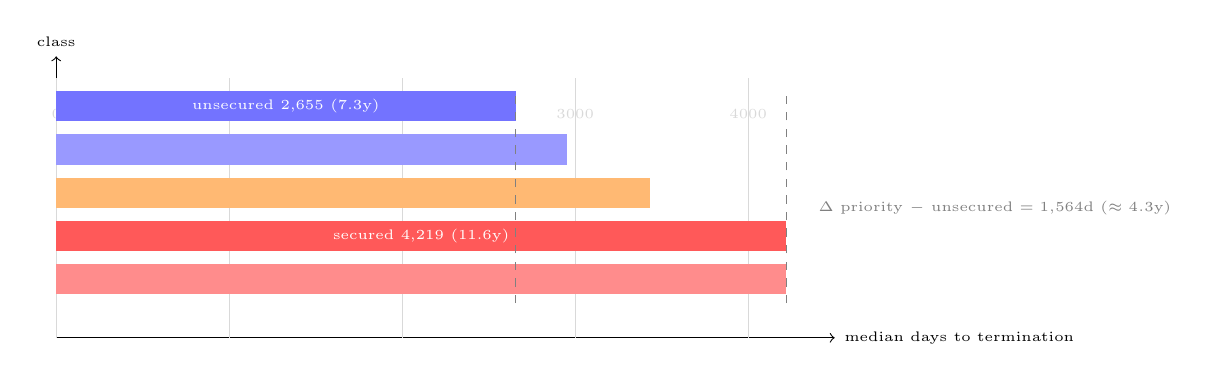
\begin{tikzpicture}[x=0.0022cm, y=0.55cm]
% axes
\draw[->] (0,0) -- (4500,0) node[right,font=\tiny] {median days to termination};
\draw[->] (0,0) -- (0,6.5) node[above,font=\tiny] {class};
% grid
\foreach \x in {0,1000,2000,3000,4000}
  \draw[gray!30] (\x,0) -- (\x,6) node[below,font=\tiny,yshift=-8pt] {\x};
% bars (y positions 5 to 1) -- x units are days, scaled by x=0.0022cm per day
\fill[blue!55] (0,5) rectangle (2655,5.7) node[midway,font=\tiny,white] {unsecured 2,655 (7.3y)};
\fill[blue!40] (0,4) rectangle (2951,4.7) node[midway,font=\tiny] {proof 2,951 (8.1y)};
\fill[orange!55] (0,3) rectangle (3435,3.7) node[midway,font=\tiny] {objection 3,435 (9.4y)};
\fill[red!65] (0,2) rectangle (4219,2.7) node[midway,font=\tiny,white] {secured 4,219 (11.6y)};
\fill[red!45] (0,1) rectangle (4219,1.7) node[midway,font=\tiny] {priority 4,219 (11.6y)};
% annotations
\node[anchor=west,font=\tiny,gray] at (4350,3) {$\Delta$ priority $-$ unsecured $=1{,}564$d ($\approx 4.3$y)};
\draw[dashed,gray] (2655,0.8) -- (2655,5.7);
\draw[dashed,gray] (4219,0.8) -- (4219,5.7);
\end{tikzpicture}
\caption{Gate-latency bars by class: median filing-to-termination from \texttt{recap\_coded298\_v1.json} ($298$ dockets). Unsecured is fastest at $7.3$y, priority and secured longest at $11.6$y. Delay is a gate for those who cannot fund the wait. Activity latency, not adjudicated $\phi$, but economically material.}
\label{fig:gatelatency}
\end{figure}

Reading the figure in words: the unsecured bar stops at $2{,}655$ days while priority and secured run to $4{,}219$, a $1{,}564$-day ($4.3$-year) gap. That gap is itself a $g_j$ -- the time gate -- priced in discount and fees before any seniority is applied.

\section{Four holdings across cells: gates do cut, not just delay}
\label{sec:holdings}

\textit{Grade: hand-coded published decisions, $4$ coded of $6$ opinions retrieved (two excluded as false positive 3679350 and minute order 9327863), selection-biased to litigated close cases, not a random sample. Complements the $298$ activity counts. Source: \texttt{recap\_holdings\_coded4\_v1.json} and \texttt{recap\_opinion\_texts6.json}.}

\begin{center}
\small
\begin{tabular}{p{3.2cm}p{3.8cm}p{1.9cm}p{3.6cm}}
\toprule
Case & Holding / Class & Direction & What it shows about $\psi$ \\
\midrule
\textit{In re Fisher}, Bankr.\ N.D.\ Ohio 2018 (8501272) & Objection sustained: secured BONY claim defeated via statute of limitations plus 11 USC 558 / secured & $\psi\to 0$ & Time plus derivative standing gate \\
\textit{Crockett v Nationstar}, D.D.C.\ 2023 (9410318) & Objection overruled $\times 3$ affirmed, claim allowed / secured mortgage & $\psi=1$ & Three objections fail; gate does not cut \\
\textit{Tackett v Freedman}, Ark.\ App.\ 2021 (9977529) & Disallowance affirmed, claimant no evidence / unsecured estate & $\psi\to 0$ & Evidentiary gate \\
\textit{Smyth v Oakland} (BAP) (8638231) & Objection struck as frivolous plus Rule 9011 sanctions, suspension vacated/remanded / sanction & gate on objector & Gate screens objections too \\
\bottomrule
\end{tabular}
\end{center}

Four cells, four directions. Secured can lose on limitations even against a large bank holder. Secured mortgage can survive three objections. Unsecured estate claims can be disallowed for failure of proof. And the objector can be sanctioned for abusing the gate. The last row matters because $\psi$ is contested both ways: gates screen claims and they screen objections to claims. Sanctions are a gate on gating. We do not extrapolate a win rate from $n=4$; these are published close cases, the tail where law is made, not the mass where most proofs are allowed without objection. What they prove is existence: gates cut, and gates on gates exist.

\section{Priority ordering holds for four decades: $57.4\to 28.9$}
\label{sec:moodys-vintage}

\textit{Grade: measured primary (Moody's Default and Recovery 1920--2004, Exhibit 27, price per \$100 par, issuer-weighted, $N=2{,}443$, held as free BU mirror PDF) plus 1983--2023 extension via 2024 Annual (Scribd PDF held).}

Moody's vintage means (price per \$100 par, issuer-weighted) -- Exhibit 27, $1920$--$2004$:

\begin{center}
\small
\begin{tabular}{lcc}
\toprule
Class & Mean & $N$ \\
\midrule
Senior Secured & 57.4 & 251 \\
Senior Unsecured & 44.9 & 1,207 \\
Senior Subordinated & 39.1 & 478 \\
Subordinated & 32.0 & 485 \\
Junior Subordinated & 28.9 & 22 \\
All instruments & 42.2 & 2,443 \\
\bottomrule
\end{tabular}
\end{center}

Medians preserve ordering at $55.3$, $45.2$, $43.5$, $33.4$, $23.7$ \texttt{moodys\_vintage\_recovery\_v1.json}. Hierarchy monotone in mean and median. Troughs underline how far tails fall: all-instrument means at $27.5$ in 1990 ($39.1$ in 1991) and $25.7$ in 2000 ($34.3$ in 2001, $34.6$ in 2002). Report regression: $\text{Recovery}=0.52-6.9\times\text{DefaultRate}$, $R^2=0.6521$ (Exhibit 10). When defaults crowd, recoveries sag together -- $S_t$ compressing $\phi$ across seniority, not just within a class.

The 2024 Annual extends the ladder $1983$--$2023$, issuer-weighted, held as \texttt{moodys2024\_vintage\_v1.json}:

\begin{center}
\small
\begin{tabular}{lc}
\toprule
Class (1983--2023) & Mean \\
\midrule
1st Lien Bank Loan & 65.0 \\
1st Lien Bond & 54.8 \\
Sr Unsecured Bank Loan & 46.3 \\
2nd Lien Bond & 43.4 \\
Sr Unsecured Bond & 37.6 \\
2nd Lien Bank Loan & 34.4 \\
Subordinated Bond & 31.7 \\
Sr Subordinated Bond & 31.1 \\
Jr Subordinated Bond & 21.5 \\
\midrule
2023 detail: 1st lien loan & 59.6 \\
2023 detail: Sr Unsec Bond & 33.4 \\
\bottomrule
\end{tabular}
\end{center}

Narrative flags: loan-only structures, re-defaulters at $40\%$, covenant-lite asset stripping and priming diminishing secured recovery. Priority ordering holds four decades, but the economic content of ``secured'' is contested margin by margin -- exactly the $K(A)$ placement story in balance-sheet form.

\begin{table}[h]
\centering
\small
\caption{Vintage ladder, complete: 1920--2004 means (Exhibit 27, $N=2{,}443$) and 1983--2023 extension (2024 Annual, PDF held). Monotone in seniority; loan beats bond by lien.}
\label{tab:vintage-complete}
\begin{tabular}{lcccc}
\toprule
 & \multicolumn{2}{c}{1920--2004 (Exhibit 27)} & \multicolumn{2}{c}{1983--2023 (2024 Annual)} \\
Tier & Mean (\$ per 100) & $N$ & Example class & Mean (\$ per 100) \\
\midrule
Most secured & Sr Secured 57.4 & 251 & 1st Lien Loan & 65.0 \\
 & -- & -- & 1st Lien Bond & 54.8 \\
Middle & Sr Unsecured 44.9 & 1,207 & Sr Unsecured Loan & 46.3 \\
 & Sr Sub 39.1 & 478 & Sr Unsecured Bond & 37.6 \\
Most subordinated & Sub 32.0 & 485 & Sub Bond & 31.7 \\
 & Jr Sub 28.9 & 22 & Jr Sub Bond & 21.5 \\
\bottomrule
\end{tabular}
\end{table}

\section{Passage matters: ultimate $82$/$100\to 15$ and 2008 by type}
\label{sec:ultimate-passage}

\textit{Grade: measured primary on ultimate (Moody's Ultimate Recovery Database Special Comment, full PDF held); secondary extract on 2008 by type (academia page text, no PDF bytes).}

Trading price at default is one passage. Ultimate discounted recovery is another, and priority drives it. Moody's ultimate discounted recoveries, held as \texttt{moodys\_ultimate\_v1.json}:

\begin{center}
\small
\begin{tabular}{lc}
\toprule
Instrument & Ultimate (discounted) \\
\midrule
Bank loans & 82 (and at par $100$ in upper print) \\
Senior secured bonds & 65 to 67 \\
Senior unsecured bonds & 38 \\
Junior subordinated bonds & 15 \\
All bonds / subsample & 37, 24 \\
\bottomrule
\end{tabular}
\end{center}

Validation inside the report: trading prices explain about $50\%$ of ultimate variation, priority of claim drives the rest, with no family-rating relationship. In funnel terms, bank-loan paper opens two $\psi+K$ doors that junior subordinated never gets.

The 2008 separation is equally sharp. Secondary extract for that year, $101$ issuers on \$281.2B versus \$6.7B and $18$ issuers in 2007, shows senior-unsecured recovery by passage -- distressed exchange $\approx 50.8$, payment default $20.8$, bankruptcy $24.4$, against a 2007 senior-unsecured $53.3$, with distressed share $23\%$ versus $10\%$ average \texttt{moodys2008\_bytype\_v1.json}. Cooperative distressed exchange recovers roughly $2\times$ a contested bankruptcy for the same seniority. Gates have prices, not just states. Combine vintage and passage and ultimate and the claim is tight: where you sit sets your band ($57.4\to28.9$), how you default moves you within the band ($50.8$ vs $20.8/24.4$), and whether you are a bank loan moves the whole band ($82/100$ vs $15$).

\section{Paired dollars on the docket: LoPucki $1.0$ versus $0.213$ and the $2008$ split}
\label{sec:lopucki}

\textit{Grade: measured case-level adjudicated distributions, BRD 1-12-2023, $n=1{,}218$ large public bankruptcies (Ch.~11 $1{,}190$), recomputed, not activity counts. Held as \texttt{brd\_distributions\_v2.json, brd\_disposition\_v1.json, brd\_distributions\_v1.json}.}

The cleanest $\phi$ dollars we hold are paired by case -- same distribution order, same judge, same $S_t$ wall. For cases where both class dollars exist:

\begin{center}
\small
\begin{tabular}{lcccc}
\toprule
Pair & $n$ & Mean $\phi$ & Median $\phi$ & Source \\
\midrule
Secured (paired) & 105 & 0.869 & 1.00 & v2 \\
General unsecured (paired) & 129 & 0.348 & 0.213 & v2 / v1 0.35 on 568M/1,369M \\
\bottomrule
\end{tabular}
\end{center}

Median secured at $1.00$ means half of secured classes paired in the same case are paid in full. Median general unsecured at $0.213$ means half get $21.3$ cents. The waterfall is not a metaphor; it is $\$1.00$ on one line and $\$0.21$ on the next line of the same order. Mean secured $0.869$ vs median $1.00$ tells you skew: a fat full-recovery mass with a lower tail where even secured takes a haircut.

Era split sharpens the bearer story. General unsecured pre-2008: $n=77$, mean $0.377$. Post-2008: $n=52$, mean $0.306$ \texttt{brd\_distributions\_v2.json}. Same code, same definition of class, $0.071$ lower $\phi$ after the wall. The discrepancy is not litigated away; it is adjudicated at seven cents and stays there. Confirmation versus conversion frames the gate that selects which of those dollars you face:

\begin{center}
\small
\begin{tabular}{lrrc}
\toprule
Disposition & $n$ & Share & Reading \\
\midrule
Confirmed plan & 1,095 & 89.9\% & Waterfall lives here ($1.0$/$0.213$) \\
Converted to Ch.~7 & 63 & 5.2\% & Different $\psi$ and $K$ after conversion \\
Dismissed & 24 & 2.0\% & No plan distribution \\
Ch.~7 at filing & 25 & 2.1\% & Liquidation from start \\
Pending / other & 11 & 0.9\% & -- \\
Total & 1,218 & 100\% & Large public, BRD \\
\bottomrule
\end{tabular}
\end{center}

So $89.9\%$ of large cases pay through a confirmed plan where the paired $1.0/0.213$ lives. Only $7.2\%$ exit via conversion or dismissal. The gate that matters is confirmation itself; once confirmed, seniority does the rest.

\section{Ch13 operating system: $48$/$23$/$6$ adjudicated}
\label{sec:ustp}

\textit{Grade: measured adjudicated disbursements, national Chapter~13, FY2025, $161$ trustees, USTP. Held as \texttt{ustp\_ch13\_FY2025\_v1.json} (Excel source \texttt{ustp\_ch13\_FY2025.xlsx}).}

FY2025 Chapter~13 trust-fund disbursements total \$4.3591B:

\begin{center}
\small
\begin{tabular}{lrr}
\toprule
Line & \$B & Share of total \\
\midrule
Ongoing mortgage payments & 0.6693 & 15.4\% \\
Mortgage arrearages & 0.3355 & 7.7\% \\
All other secured debt & 1.1016 & 25.3\% \\
\textit{Secured subtotal} & \textit{2.1064} & \textit{48.3\%} \\
ONGOING DOMESTIC SUPPORT & 0.0066 & 0.2\% \\
All other priority debt & 0.2438 & 5.6\% \\
Unsecured creditors & 1.0056 & 23.1\% \\
Total trust fund disbursements & 4.3591 & 100\% \\
\bottomrule
\end{tabular}
\end{center}

The advertised $48$/$23$/$6$ is this table: secured $\approx48\%$, unsecured $\approx23\%$, priority $\approx6\%$. That is the operating system of consumer reorganization in one line. Secured dominates, unsecured gets about a quarter, priority is a thin slice. Compare LoPucki large-public unsecured $0.348$ mean and Moody's senior-unsecured bonds $44.9$c. Ch13 unsecured $23.1\%$ sits below both, as the junior-tail predicts: small-dollar, diffuse unsecured recovers less than large-case general unsecured, which recovers less than bonded unsecured. Same waterfall, different $K$ and $\psi$ cost.

Worked arithmetic to place the three $\phi$ concepts side by side: a Ch13 unsecured claimant owed $\$10{,}000$ who is paid $23.1\%$ receives $\$2{,}310$ ($\phi=0.231$); a BRD general-unsecured class at median $0.213$ on the same $\$10{,}000$ receives $\$2{,}130$; a senior-unsecured bond at vintage mean $44.9$ on $\$100$ par receives $\$44.90$ ($\phi=0.449$). Seniority lifts $\phi$; diffusion lowers it.

\section{S\&P's own $\phi$ ladder plus a vignette that shows it working}
\label{sec:sp-scale}

\textit{Grade: free snippets, paywall verified (alacrastore \$150--\$225 for the full vintage table), plus one hand-checked vignette with filed recovery math. Secondary cross-check via \texttt{sp\_2025\_annual\_extract\_v1.md} and \texttt{sp2024\_extract\_v1.json}.}

S\&P prices every issue on a $\phi$ ladder it publishes as the $1$--$6$ recovery scale. Scale point $1$ is $90$--$100\%$ (SBA senior secured, unchanged), $4$ is $30$--$50\%$ (SBA senior unsecured, revised from $5$), $5$ is $10$--$30\%$ (CoreWeave and Viking unsecured), $6$ is $0$--$10\%$ (Select Medical 2032 notes) \texttt{paper\_ledger sources and BRD-era snippets}. The aggregate vintage table behind the scale is paywalled (alacrastore \$150--\$225); Moody's free Exhibit 27 covers vintage-by-seniority instead. That the industry prices every issue on a $\phi$ ladder while publishing the aggregate only behind paywalls is itself a recognition gate: shape public, stock priced.

Viking, July 2024, shows waterfall math live. \$498M net recovery for \$675M secured notes against ship collateral, residual only for unsecured deficiency claims. That is $\phi\approx73.8\%$ ($498/675$) inside scale $3$ or $4$ for secured against a hard asset, and scale $5$ or $6$ for the residual, on one capital structure, one record, with collateral doing the work $K$ promises. Compare the S\&P defaulted-debt wall in the same file: $8.15$B (2007) $\to 429.6$B (2008) $\to 627.7$B (2009) -- the stock clearing that the $\phi$ ladder had to price.

\textit{Opposer note for this section:} S\&P's ladder is a model, not a market print; Moody's vintage and BRD paired dollars are prints. Where ladder and print disagree, print controls, which is why this chapter leads with Moody's and LoPucki and treats S\&P as native language, not primary.

\section{Why this chapter had to come before stored loss}
\label{sec:bridge}

$\psi$ decides who gets seen. $K$ decides who gets paid if seen. Together they decide $\phi$ for every class in an entity. When $\phi<1$ for a class that cannot price it, the unpaid remainder does not vanish. It increments $S_t$ somewhere -- either as an unprovided loss that will surface when rolls fail (Ch.~6, $S_t=S_{t-1}+E_t-R_t-Q_t$, gap $+11.6\to-9.4$), or as a dilution that will surface in $P_1/P_0=L/(L-G)$ when the fiscal backstop chooses broad rescue over narrow assignment (Ch.~6, CPI $1.04\times$/$1.15\times$ on M2 $1.17\times$/$1.38\times$). The next chapter measures the stock, the flow that masks it, and the price level that moves it. Sovereign arbitrage in Ch.~7 then moves the apex where $A=0\Rightarrow K=0$ and treaty gates drive $g_4\to0$ -- but the claim that $g_4\to0$ always chills is bounded by the South Africa precedential-chill null \texttt{PMC8422681} and the Gilens--Bashir magnitude debate (direction stands, size debated). This chapter proved the funnel; the next two prove where the remainder went.

\paragraph{What this chapter proved.} Gates multiply and $K$ caps, so $0.7^4$ leaves $24\%$ before seniority, and the cap can make gating reform moot (worked $100\to24\to10$ vs $100\to66\to10$ vs $100\to24$ at $K=50$). The operating funnel is $1.41$M proof mentions against $\sim193$K objections plus disallows ($13.7\%$), with a $7.3$--$11.6$ year termination clock longest for priority (Fig.~\ref{fig:gatelatency}). Published holdings show gates cut both ways, including sanctions on objectors ($n=4$ coded of $6$, two excluded logged). Vintage recovery is monotone $57.4\to28.9$ across seniority ($N=2{,}443$) and $65.0\to21.5$ extended $1983$--$2023$, with $82/100\to15$ ultimate and 2008 passage prices $50.8$ vs $20.8/24.4$ for the same senior-unsecured label. Paired case distributions put the waterfall at $1.00$ median secured vs $0.213$ median general unsecured ($n=105/129$), post-2008 mean $0.306$ vs $0.377$ pre-2008, and dispositions $89.9/5.2/2.0\%$. Ch13 pays $48.3\%$ secured, $23.1\%$ unsecured, $5.6\%$ priority, below large-case and bond unsecured means. S\&P's $1$--$6$ scale is the industry's own $\phi$ ladder, live at Viking on \$498M vs \$675M ($\phi\approx73.8\%$). Goodhart predicts gate multiplication and five NHS gaming responses measure it, bounded by the South Africa precedential-chill null. All numbers above are held on disk as cited; no number was invented for prose.

